\documentclass{article}
\usepackage{fullpage,amsmath,amsthm,graphicx,enumitem,amssymb}
\usepackage[hidelinks]{hyperref}
\theoremstyle{definition}
\newtheorem{thm}{Theorem}
\newtheorem{question}[thm]{Question}
\newenvironment{solution}{\noindent\textit{Solution:}}{}

\newcommand{\reals}{\mathbb{R}}

\title{ASEN 6519-007 Decision Making under Uncertainty\\
       Homework 2: Markov Decision Processes}

\begin{document}

\maketitle

\section{Conceptual Questions}

\begin{question}
    Give an example of an MDP with a unique nonzero optimal value function, but multiple optimal policies.\footnote{Hint: you can do this with $|\mathcal{S}| = 1$.}
\end{question}

\begin{question}
    Consider a stationary infinite-horizon MDP with $\mathcal{S} = \{1,2\}$, $\mathcal{R}(s, a) = s^2$, and $\gamma = 0.9$ ($\mathcal{A}$ and $\mathcal{T}$ are unknown). Suppose that policy $\pi$ achieves a value at state $1$ of $V^\pi(1) = 37$. What is $V^*(2)$, the optimal value at state $2$? Justify your answer.
\end{question}

\section{Exercises}

\begin{question}
    Consider a 1 by 9 grid world with a key in cell 2 and a locked door in cell 8. An agent automatically enters the door and receives a reward of 10 upon returning to cell 8 after having collected the key, and the problem terminates immediately. At each time step, the agent can take one of two actions, \texttt{left}, or \texttt{right}. 90\% of the time, the action succeeds and the agent moves in the desired direction; 10\% of the time the agent moves in the opposite direction. If an end wall is hit, the agent bounces back to the previous cell. The discount factor is $\gamma=0.95$.
\begin{center}
    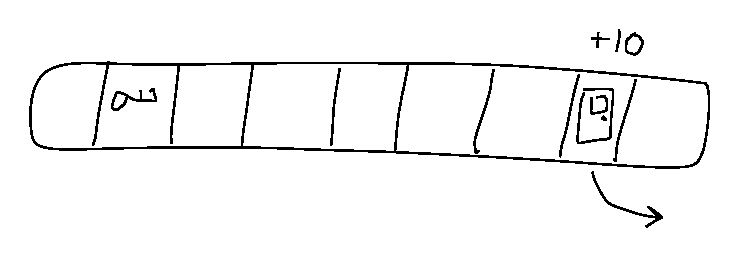
\includegraphics[width=0.5\textwidth]{small_mdp.pdf}
\end{center}

    Formulate this problem as an MDP, and write down the state space $\mathcal{S}$ and reward function $\mathcal{R}$. What is the value of being in cell 9 without the key (report with a precision of 0.001)?

    % TODO: add picture
\end{question}

\begin{question}

    Consider a continuous state and action MDP with $\mathcal{S} = \reals$, $\mathcal{A} = \reals$, $R(s, a) = - 2s^2 - a^2$ and transitions described with the generative model $s' = G(s, a, w) = 2s + a + w$ where $w$ is a normally-distributed random variable with zero mean and variance $1$. Optimal control theory\footnote{\url{https://en.wikipedia.org/wiki/Linear\%E2\%80\%93quadratic_regulator}} tells us that an optimal policy for this problem with the undiscounted time-average objective has the form $\pi^*(s) = -k\,s$ where $k$ is a real number. Find $k$ for the optimal policy to a precision of 0.02.\footnote{Hint: The most straightforward way to do this is with Monte Carlo policy evaluation and brute force search. If you know how to formulate and solve this as an optimal control problem, you may also use that method.}
\end{question}

\section{Challenge Problem}

\begin{question}
    Value iteration for ACAS given $\mathcal{T}$ and $\mathcal{R}$.

Your task is to find the optimal value function for an Aircraft Collision Avoidance System (ACAS). The encounter model will be specified as a Markov decision process, and your task will be to compute the value function using value iteration or another suitable algorithm. The continuous physical state space will be discretized at various levels of granularity and the goal is to find the value function for the finest discretization possible.

For this exercise, you may NOT use any outside libraries designed specifically for solving MDPs such as POMDPs.jl solvers, though you may look to them for inspiration.

A model with discretization level \texttt{n} can be constructed with
\begin{verbatim}
                        m = DMUStudent.HW2.UnresponsiveACASMDP(n)
\end{verbatim}
The higher \texttt{n} is, the finer the discretization and the larger the state space. Transition matrices for each of the 3 actions can be constructed with \texttt{T = transition\_matrices(m)}. This returns a dictionary that contains a transition matrix for each action. For example \texttt{T[1][2,3]} is the probability of transitioning from state 2 to state 3 when action 1 is taken. Reward vectors for each action can be constructed with \texttt{R = reward\_vectors(m)} where \texttt{R[1][2]} is the immediate reward of taking action 1 in state 2.
The discount factor for the problem is $\gamma = 0.99$.

The score received for solving the problem is \texttt{n}. You must submit your score to the leaderboard at \url{http://dmuleaderboard.com/hw2}. A score of \texttt{n} = 7 will receive full credit.

\vspace{1em}
\noindent\makebox[\linewidth]{\rule{\textwidth}{0.4pt}}
\vspace{1em}

\textbf{The only information strictly necessary to solve the problem is the transition matrices and reward vectors mentioned above.} However, the description of the model below may help to get the highest score on the leaderboard. The continuous model is defined as follows:

\begin{center}
    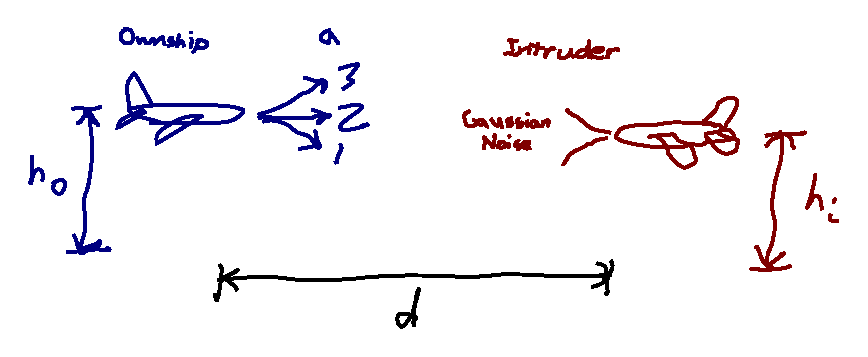
\includegraphics[width=0.7\textwidth]{unresponsive_acas.pdf}
\end{center}

\begin{itemize}
    \item The state space is 4-dimensional $\mathcal{S} = \reals^4$, with each state consisting of $s=(h_o, \dot{h}_o, h_i, d)$ where $h_o$ is the ownship altitude in feet, $\dot{h}_o$ is the rate of climb in ft/min, $h_i$ is the intruder altitude in feet, and $d$ is the distance between the aircraft in feet. An integer state \texttt{s} can be converted to a vector that shows the values of these variables using \texttt{POMDPs.convert\_s(ACASState, s, m)}.
    \item The action space is $\mathcal{A}=\{1,2,3\}$. $a=1$ represents decreasing the rate of climb $\dot{h}_o$ by 1500 ft/min, $a=3$ means increasing the rate of climb by 1500 ft/min, and $a=2$ means maintaining the same rate of climb. The possible rates of climb are $\dot{h}_o \in \{-3000, -1500, 0, 1500, 3000\}$
    \item A reward of -100 is received for a near-mid-air collision, defined as the aircraft passing within 500 vertical feet and 100 horizontal feet of each other. Any change in rate of climb yields a reward of -1.
    \item The rate of climb, $\dot{h}_o$ changes instantly when an action is applied. Then the following dynamics are used: $d' = d - 2\,v\,\Delta t$ where $v$ is the fixed horizontal velocity, $h_o' = h_o + \dot{h}_o\,\Delta t$, and $h_i' = h_i + W_{\Delta t \sigma^2}$ where $W$ is the Wiener process\footnote{\url{https://en.wikipedia.org/wiki/Wiener_process}}. $\Delta t$ changes based on the discretization \texttt{n}.
\end{itemize}

The model \texttt{m} implements the POMDPs.jl explicit MDP interface\footnote{\url{https://juliapomdp.github.io/POMDPs.jl/stable/explicit/\#Explicit-(PO)MDP-interface-1}}, and students are welcome to explore the problem further using that interface as well as ask on Piazza and look at the source code for details.

\end{question}

\end{document}
